\documentclass [oneside, a4paper, openany]{book}


\usepackage[utf8]{inputenc}
\usepackage[british]{babel} % Use British english for hyphenation etc
\usepackage{tocbibind} % Auto add Bibliography etc to Table of Contents
\usepackage[round]{natbib} % Use BibTeX for bibliography management
\setcitestyle{notesep={: }} % Sets the cite separator to column instead of comma
\usepackage{graphicx}
% \usepackage{tikz} % Inline drawing
\usepackage{tabu} % Easier longtables
% \usepackage{url}
\usepackage{hyperref} % Create hyperlinks within text
\usepackage[toc,nonumberlist,nopostdot]{glossaries}

\makeglossaries % Creates the glossary section

\graphicspath{{./assets/}}
\begin{document}

\frontmatter
\begin{titlepage}
  \newcommand{\HRule}{\rule{\linewidth}{0.5mm}}
  \center

  \textsc{\LARGE Robert Gordon University}\\[1.5cm]
  \textsc{\Large Bachelor of Science in Computer Graphics and Animation}\\[0.5cm]
  \textsc{\large Honours Project Report}\\[0.5cm]

  \HRule \\[0.4cm]
  { \huge \bfseries A Mobile Application that applies Self-Management Approach to Reduce Sedentary Behaviour}\\[0.4cm]
  \HRule \\[1.5cm]

  \begin{minipage}{0.4\textwidth}
  \begin{flushleft} \large
  \emph{Author:}\\
  Georgi \textsc{Koemdzhiev}
  \end{flushleft}
  \end{minipage}
  ~
  \begin{minipage}{0.4\textwidth}
  \begin{flushright} \large
  \emph{Supervisor:} \\
  Dr. Stewart \textsc{Massie}
  \end{flushright}
  \end{minipage}\\[4cm]

  {\large 2017}\\[3cm]

  
\includegraphics[width=5cm, scale=0.1]{rgu-logo.png}\\[1cm]
  \vfill
\end{titlepage}
\chapter{Declaration}
I confirm that the work contained in this Honours project report has been composed solely by myself and has not been accepted in any previous application for a degree. All sources of information have been specifically acknowledged and all verbatim extracts are distinguished by quotation marks.\\[2cm]

  \noindent Georgi Koemdzhiev\\
  \today
\chapter{Abstract}
Sedentary behaviour is a leading cause of numerous chronic deceases but currently there is a lack of mobile applications that try to help tackle this problem. The purpose of this paper is to show how behaviour change techniques can be applied in a mobile application to help people change their sedentary habits. This project proposes a smartphone application that uses activity daily guidelines to increase physical activity. This software will be developed based on findings from background research. It will incorporate behaviour change techniques that will allow maintaining a good goal-performance relationship. Also, self-management logic will be present to facilitate self-care features such as setting a psychical activity goal.
\chapter{Acknowledgements}
  to be done

\setcounter{tocdepth}{1}% Allow only \chapter in ToC
\tableofcontents
\listoffigures
\listoftables

\newglossaryentry{har}
{
  name=HAR,
  description = {Human Activity Recognition}
}

\newglossaryentry{gsc}
{
    name=GSC,
    description = {Goal-Setting Component}
}

\newglossaryentry{mc}
{
    name=MC,
    description = {Monitoring Component}
}

\newglossaryentry{fc}
{
    name=FC,
    description = {Feedback Component}
}

\newglossaryentry{pa}
{
    name=PA,
    description = {Physical Activity}
}

\newglossaryentry{st}
{
    name=ST,
    description = {Sedentary Time}
}

\newglossaryentry{sb}
{
    name=SB,
    description = {Sedentary Behaviour}
}

\newglossaryentry{mvp}
{
    name=MVP,
    description = {Model View Controller is a design pattern that separates the software logic into tree roles: model, view, or controller}
}

\newglossaryentry{ui}
{
    name=UI,
    description = {User Interface}
}

\newglossaryentry{sa}
{
    name=SA,
    description = {System Architecture}
}

\newglossaryentry{ide}
{
    name=IDE,
    description = {Integrated Development Environment}
}

\newglossaryentry{fft}
{
    name=FFT,
    description = {Fast Fourier Transform is an algorithm that converts a signal from its original domain (often time) to a representation in the frequency domain}
}

\glsaddall %Print all entries %
\setglossarystyle{altlist}
\printglossaries

\mainmatter
\chapter{Introduction}
\label{Chapter:Introduction}
Nowadays, with the rapid advance of technology people spend a lot of their time in a static position. According to \citet{wilmot2012} that increases the chances of all-cause mortality by 49\%.  Also, people who lead non-active lifestyle are 112\% more likely to get diabetes, 147\% more likely to experience cardiovascular events, and 90\% more likely to die due to cardiovascular events. 
    
Using self-manageing systems to counter sedentary behaviour is becoming a well-accepted solution due to its many advantages over the traditional paper based methods. This paper proposes a self-management mobile application that apples behaviour change logic to reduce sedentary time as well encourage more physical activity. 
    
    \section{Project Catalyst}
    My passion for software began back in my first year as a student at Robert Gordon University. I was exposed to various modules related to software development which I found absorbing. Consequently, I was able to do a summer internship with a company called xDesign as a Software Engineer and thus gain industry knowledge and skills. I was confident that mobile application development was an area I wanted to pursue. 
    
    This passion for software contributed immensely on the topic of my honours project. Also, the idea of the health aspect of the mobile application made the subject even more appealing to me. My application could potentially help people self-manage their sedentary time as well as promote more physical activity using only the build-in accelerometer sensor on a smartphone. 
    
    
    \section{Aims and Objectives}
    A set of goals and objectives were formed prior to the initiation of the project to help shape its scope. The goals of the project define the main motivation behind it whereas the objectives underline the main tasks that the project undertakes.
    
    \subsection*{Aims}
    The following project goals have been identified: 
    \begin{enumerate}
        \item Develop a fully working \gls{har} system
        \item Incorporate the above within a \gls{sb} self-manageing system
        \item Evaluate the system performance using user feedback
    \end{enumerate}
    
    \subsection*{Objectives}
    The following list of objectives helped accomplishing the above goals: 
    \begin{enumerate}
        \item Investigate and gather information about \gls{har} on wearable devices
        \item Research the effects of \gls{sb}
        \item Investigate behaviour change approaches
        \item Design and implement a \gls{har} and Self-management systems
        \item Design and implement a mobile application on the Android platform incorporating the above systems 
    \end{enumerate}
    
    \section{Document structure}
    This section of the document addresses how this report is organised.\newline
    
    \textbf{Literature Review} Gives a wide background information regarding using self-management technologies in the health sector, Behaviour changing techniques, consequences and current situation of of Sedentary Behaviour as well as researching commercial and non-commercial HAR mobile applications.\newline
    
    
    \textbf{Specification} Lists the proposed mobile application Functional and Non-functional requirements as well as discussing the system quality attributes. The information in this chapter is heavily influenced by the \textit{Literature Review} chapter.\newline
    
    
    \textbf{Design} Addresses the system design decisions\newline
    
    
    \textbf{Implementation} Details about how the system design have been implemented for each of the main system components.\newline
    
    
    \textbf{Evaluation} A discussing how effective is the implemented system on users.\newline
    
    
    \textbf{Conclusion} Summary of the potential benefits of Sedentary Behaviour self-manageing devices in the health sector, future work and project critical appraisal.\newline
    
    
    \section{Professional, Social, Ethical, Security and legal issues to the project}
    
    \subsection{Professional}
    As a student studying Computing for Graphics and Animations – a course that is accredited by the British Computer Society (BCS) I intend to comply with the BCS Code of Conduct. Especially, point 4 (d) \citep{bcs_2017} - “act with integrity and respect in your professional relationships with all members of BCS…”. Thus, I intend to acknowledge the work of all external software authors used in this work (see Appendix \ref{chapter:third-party-software}).

    \subsection{Social}
    The proposed application will try to avoid promoting any body image stereotypes by focusing more on encouraging the users to be more active rather than on their body characteristics such as weight and height or BMI (Body Mass Index). In addition, the application will only show what the recommended activity intervals per day are and will not force the users of the application to follow those strictly (some jobs do require seating for extended intervals of time – e.g. Pilots).
    
    \subsection{Ethical}
    The data collected during the project development such as names of the project participants and their accelerometer sensor data will be stored on disk only for the development purposes of the project. 
    
    \subsection{Security}
    The mobile application, proposed in this work, will offer an authorisation component to prevent other people accessing personal data such as total minutes of activity/inactivity collected daily. What is more, any relevant or valuable user data will be anonymised to protect individual’s identity.

    
    \subsection{Legal}
    To prevent any harm done to the user, the mobile application will show a disclaimer (warning) dialog message to inform the user that they should be in a good physical condition (not suffering from diseases that could lead to worsening the condition of the user) before they use the application. In addition, I intend to fully comply with the terms of conditions of any third party software that I intend to use (my main goal is to use primarily Open Source software). As far as the project participant’s data is concerned, I intend to keep the data only for the purposes of this project, and the data will not be used for any commercial purpose. 

\chapter{Literature Review}
\label{Chapter:Literature-Review}

As it was mentioned in Chapter \ref{Chapter:Introduction} this document proposes a system implemented on a mobile device that encourages the reduction of sedentary time via self-management techniques. In order to gain knowledge on how to devise such as system, literature review needs to be carried away on several topics. First of all, the current shift towards self-management in the health sector will be discussed. The next section will focus on evaluating how much time people spend in Sedentary Behaviour (SB) and what are the consequences. Section 3 looks at digital behaviour change techniques. Commercial and non-commercial \gls{har} mobile applications and \gls{har} itself are discussed in Section 4. Section 5 summarises the system proposed.

\section{Self-Management in the Health Sector}
 \label{section:sm-in-hs}
    Mobile devices with embedded self-management logic are currently being utilised and becoming a well-accepted solution for millions of people in the health sector. For example, the NHS’s England Executive – Simon Stevens, launched a programme “Test Beds” \citep{nhsengland2016,nhsengland2016a} which is a set of collaborative projects between NHS and some technology companies such as Verily, IBM and Philips. The idea behind the project is to test the effectiveness of different technological innovations, including wearable devices and mobile applications. These technologies will enable patients to self-manage illnesses such as diabetes, heart diseases and dementia.
    
    \subsection{Advantages of self-management}
    Shifting towards self-care via mobile devices has many advantages over the traditional methods (e.g., over the phone or face-to-face). For example, self-care devices enable patients to monitor their illnesses at home. \citet[10]{roberts2006} finds that patients using wearables improve their condition and shorten their recovery time if they can be in a familiar environment. Real-time feedback is another advantage of using self-management devices. For example, \citet{alivecor2016}, can prevent critical and even fatal incidents by identifying illness clues ahead of time. Thus, the number of patients becoming seriously ill or needing hospital treatment will potentially be reduced. Consequently, that could save money on hospital treatments \citep{campbell2016}. In addition, \citet[6]{shuger2011} found that real-time feedback on \gls{sb} could be beneficial for weight loss. \citet[97]{whitehead2016} concludes that self-management approaches delivered via mobile applications have the potential to improve outcomes of many chronic diseases.
    
    \subsection{Need for self-management devices}
    It has been found that there is a gap in the current market regarding self-care devices that focus on monitoring \gls{sb} and not only \gls{pa}. For example, \citet{sanders2016} found out that there is a lack of self-management mobile applications or devices on the market that can monitor \gls{pa}. After research, he was able to find 73 devices that provide self-monitoring of PA, and only 9 can monitor sedentary time (see Figure \ref{fig:devices-to-provide-SB-feedback}). That means that there is a lack of products in the market that offer self-management of SB in addition to PA. Sanders also concluded that the current devices capable of measuring sedentary time and providing feedback have not been used in behaviour change interventions. In conclusion, there is a need for further research and development of self-care enabled wearables to help people engage in behaviour change interventions and prevent possible chronic diseases. 
    
    \begin{figure}[h]
        \centering
        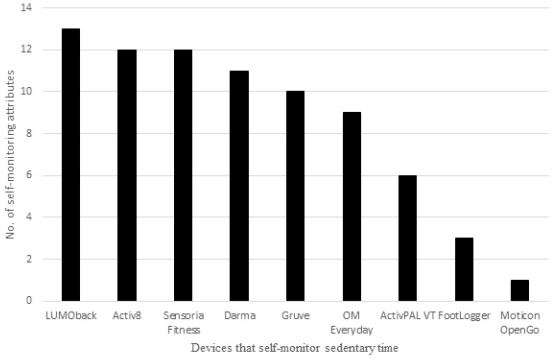
\includegraphics[width=10cm]{figureOne}
        \caption{Current technologies that self-monitor and provide feedback on SB \citep{sanders2016}}
        \label{fig:devices-to-provide-SB-feedback}
    \end{figure}

\section{Sedentary Behaviour}

Understanding the consequences of \gls{sb} as well as recommended daily energy expenditure levels is crucial for developing a mobile application that aims to implement behaviour changing theory. It is said that there is a difference between \gls{sb} and \gls{pa} and these terms should be treated differently \citep[540]{networ2012}. For example, a person can do both be sedentary for prolonged periods of time and spend large amounts of vigorous physical activity in one day. Networ define \gls{sb} as “energy expenditure less or equal to 1.5 METs while in a sitting or reclining posture” (see Table 1 for comparison of different activities). As it can be seen from Table \ref{tab:activity-intensities}, the energy spent in static activities does not result in a lot of energy expenditure and that potentially could lead to the occurrence of chronic diseases. \citet[540]{networ2012} also defines a person who is “inactive” as “not meeting specified physical activity guidelines”. That means that a person has to meet the PA recommendation levels in order to be considered as active. The next section will discuss the consequences of SB and the suggested amount of physical activity per day.
    
    \begin{table}[h]
        \centering
        \begin{tabular}{c}
            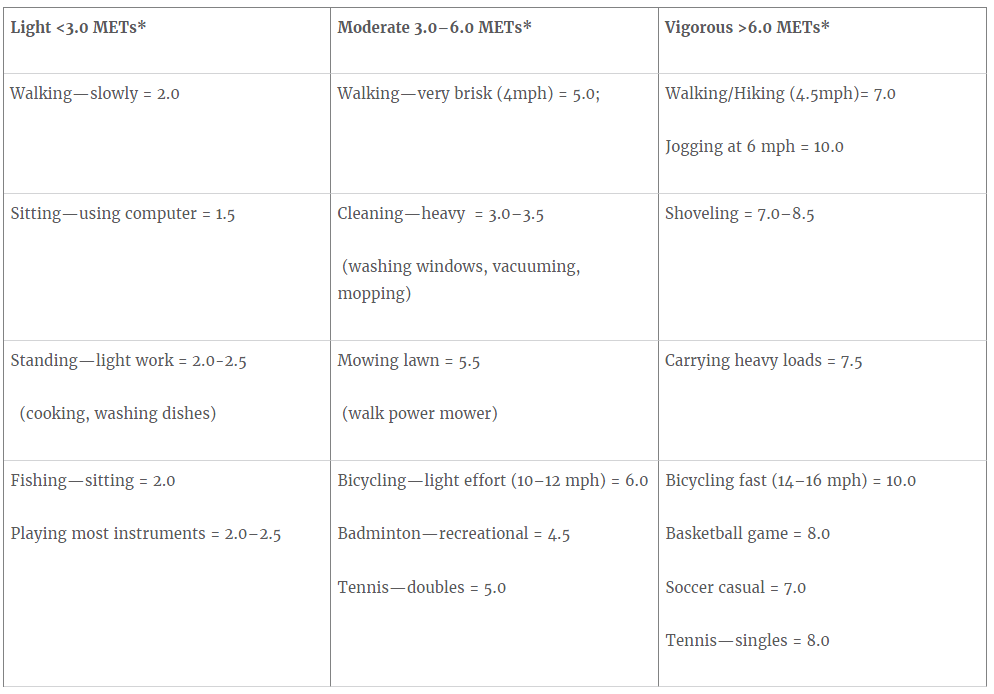
\includegraphics[width=10cm]{tableOne}
        \end{tabular}
        \caption{Examples of light, moderate, and vigorous activities}
        \label{tab:activity-intensities}
    \end{table}
    
    \subsection{SB consequences and PA recommendations}
    Sedentary Behaviour has been positively associated with diseases such as back pain, diabetes, cardiovascular disease, cancer and all-cause mortality (Wilmot et al., 2012: 2895–2905, Biswas et al., 2015: 123 and Department of Health, 2010: 18). In addition, Biswas et al. (2015: 127) even concluded that SB causes adverse outcomes regardless of the physical activity, although the chances of developing a SB associated chronic diseases are low when involved in higher levels of physical activity.
    
    As far as the PA recommendations are concerned, the Department of Health (2011) and Townsend et al. advocate for 30 minutes of PA for every day of the week. What is more, Parkinson (2016) and Siddique (2016) state that an ideal PA per day would be an hour. Having said that, simply doing 30 minutes or even an hour of activity is not enough. For example, a person may do 30 minutes of activity a day and spend the rest of the time laying or sleeping. To counter that, Swartz, Squires, and Strath (2011) suggest that every static hour should be interrupted by at least of a five-minute walk.
    
    \subsection{Current statistics of sedentary behaviour}
    \citet[19]{townsend2015} found in 2012 that 34\% of adult man and 46\% of adult women did not meet the recommended levels of physical activity. Also, according to \citet[81]{townsend2015}, 45\% of the adults in the UK spend up to 5h and 30 minutes in SB such as watching TV, using a computer or playing video games. What is more, \citet{swinford2014} found in a survey that there has been an increase in the time people spend in sedentary activities compared to 1995. For example, he found that people nowadays take 18 per cent fewer journeys, 24 per cent fewer go to do shopping and 28 per cent visit friends compared to 1995. In conclusion, to improve the state of the people who are spending too much time in sedentary behaviour, there is a need for further research on the effectiveness of behaviour change interventions only focusing on sedentary time and physical activity alone \citep[130]{biswas2015}.

\section{Behaviour change}
Behaviour change is a critical aspect of self-management. It could encourage and motivate people who spend too much time being sedentary to improve their lifestyle. Behaviour change includes the following main components: goal-setting, monitoring and feedback. \citet[191]{strecher1995} find that setting a specific goal, combined with performance feedback, increases task performance (how well a task is achieved) when compared to having no goal or non-quantitative goal such as “do you best”.

Providing feedback is also important in order to successfully implement behavuour change. \citet[708]{locke2002} gives the following example “If the goal is to cut down 30 trees in a day, people have no way to tell if they are on target unless they know how many trees have been cut”. A person needs to know how much effort they need to put in order to attain a previously set goal. This information is provided by the monitoring component of the behaviour changing circle, which know what \gls{pa} and \gls{sb} amounts the user has accumulated at a given time.
    
    \subsection{Goal-setting reliability requirements}
    \citet[191]{strecher1995} state that goal-setting does not evoke motivation automatically. For instance, a person has to be interested in achieving the goal in the first place or, otherwise, the effect of setting a goal will be small or the whole process may turn out to be counterproductive. In addition, they claim that it is possible for a person to fail to attain a goal even though they are interested in achieving it. For example, the goal of becoming more active and less sedentary could conflict with the goal of quitting smoking. However, if there is no significant conflict, goal setting is a viable method for achieving one’s motivation towards behaviour change. What is more, \citet[714]{locke2002} rounds out this idea by stating that the goal-setting method is very reliable and it could fail only if some of the task-performance mediators are not executed properly.
    
    \subsection{Goal-performance moderators}
    Three moderators\footnote{A moderator is variable that affects the relationship of two other variables (Moderator mediator, no date). For example, in the case of behaviour change a moderator would affect the goal the user set (i.e. become less sedentary) and task performance (how well the person achieves this).} have been found to be involved in the goal-performance relationship – \textbf{commitment} (directly affected by the importance of the goal and the self-efficacy\footnote{\textit{Self-efficacy can be described as "the belief in one’s capabilities to organize and execute the courses of action required to produce given attainments}" \citep[308]{williams2011} (quotes Bandura A, 1997)}), \textbf{feedback}, and \textbf{difficulty} \citep[707]{locke2002}. Those moderators are widely used today in the modern health tracking wearables to increase the level of engagement and motivation.
    
    The goal \textbf{commitment} moderator is affected by both the importance of the task and the self-efficacy of the user. It has been found that making a goal public increases the \textbf{importance} of a task since ‘it makes one’s actions a matter of integrity in one’s own eyes and in those of others’ \citep[707]{locke2002}. For example, \citet[]{endomondo2016} – a sport tracking mobile application allows public sharing of workouts data, tagging friends and an option to challenge or get challenged by friends. Also, \citet[708]{locke2002} state that commitment is also affected by the \textbf{self-efficacy}. For example, finding “models” that a person can relate to by providing the users with the ability to see how they compare to users with similar performance (Endomondo).
    
    What is more, \citet[708]{locke2002} found that providing feedback on the goal attainment progress affects the goal-performance relationship. Without knowing the current progress towards the goal, it is difficult for the user to adjust the effort. For example, mobile applications such as Endomondo and Runkeeper \citep{fitnesskeeper2016} provide \textbf{feedback} on the goal progress to keep the user informed about their goal-performance.
    
    Last but not least, goal \textbf{difficulty} also affects the goal-performance relationship. \citet[709]{locke2002} concluded that people who can set their goals usually set higher goals and that is associated with better performance than pre-assigned goals (Mitchell, and Dossett, 1978 cited in Locke and Latham, 2002: 709). For example, today’s mobile fitness applications allow the user to set goals \citep{fitnesskeeper2016,endomondo2016} so how challenging the goal is depends on the user.
    
\section{HAR enabled mobile applications}
\gls{har} is a crucial technology due to its many applications in self-management. It is involved in the monitoring stage, after setting a goal, and performs the recognition of activities such as walking using sensor data. This section will discuss the general approach to developing a \gls{har} enabled system that detects different types of ambulation activities (e.g., walking and running) as well as explore commercial and non-commercial \gls{har} enabled mobile applications (and devices) in the market. The non-commercial \gls{har} solutions will be discussed regarding \textit{sensor type and location}; \textit{feature extraction and learning algorithm; accuracy and energy consumption}. Next, the commercial products will be discussed with regard to what attributes are gathered.

    \subsection{Design of a HAR system}
    Depending on the learning method, \gls{har} systems can be categorised into supervised or semi-supervised (see figure \ref{fig:design-of-har}). Supervised HAR systems require labelled data set to train a classifier. Supervised \gls{har} systems can also be classified as, according to the response rate, online and offline \citep[29]{labrador2013}. The former provides real-time feedback to the user. The latter \gls{har} systems are indented for applications that do not require immediate feedback due to high computations or the need of remote application server. \gls{har} systems usually require two initial stages – training and testing \citep[4]{labrador2013}. During the training state, time series dataset is provided (see figure \ref{fig:har-data-flow}). Time series data  commonly is divided into time windows (e.g. 3 seconds) that contains the raw measurements of sensors. Future extraction algorithms are then applied to each time window in order to extract valuable information from the data (i.e. features). Later, different learning algorithms are used to generate a \textit{classifier} based on the extracted features. The classifier can then classify “unseen” or unlabelled data into activities such as walking or running. 
    
    \begin{figure}[ht]
        \centering
        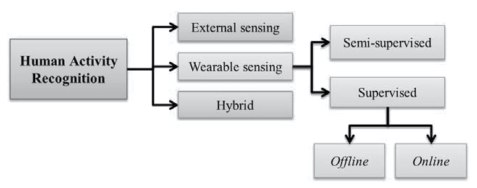
\includegraphics[width=10cm]{design-of-har-systems}
        \caption{General design of HAR systems}
        \label{fig:design-of-har}
    \end{figure}
    
    \begin{figure}[ht]
        \centering
        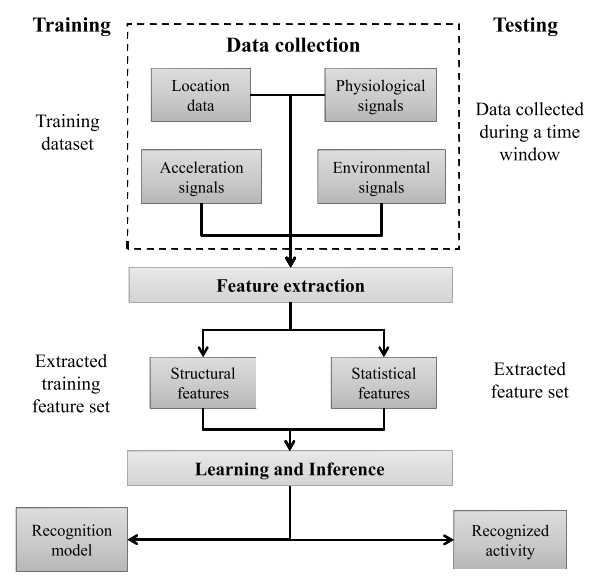
\includegraphics[width=8cm]{training_testing_har}
        \caption{General HAR system data flow}
        \label{fig:har-data-flow}
    \end{figure}

    \subsection{Non-Commercial HAR systems}
    
    The development of \gls{har} systems date back to the 90s, but there is still need for improvement regarding battery consumption, obtrusiveness, and accuracy \citet[29]{labrador2013}. Good example of \gls{har} systems are \textit{Vigilante} \citep[38-39]{lara2012}, \textit{ActiServ} \citep{berchtold2010} and COSAR \citep[271-289]{riboni2010}.
    
        \subsubsection{Sensor type and location}
        Current and past \gls{har} systems have been successfully implemented using one or many sensors. For example, based on system called \textit{Centinela} \citep[38]{lara2012a}, \textit{Vigilante} uses a sensor strap attached on the chest of the user that measures 3D acceleration and six vital signs such as heart rate, respiration rate and others. Also, there are systems that utilise just one sensor \citep[1-3]{paul2015}. In addition, \citet[1-4]{torreshuitzil2015} proposed a system that uses only the embedded accelerometer sensor on a smartphone and did not restrict the user of keeping the device in a specific location.
        
        The placement of the sensors is critical and affects the accuracy grammatically. \citet[2245–2250]{he2008} concluded that the optimal position of the sensor is inside the trousers pocket since it is convenient. However, \citet[1194]{lara2013} found that the position of the sensors depends on the application of the \gls{har} system and the activities to be recognised. For example, placing an accelerometer on the wrist may introduce errors in the data due to incidental arm movements.
        
        \subsubsection{Feature extraction and feature selection}
        As it can be seen in Figure \ref{fig:design-of-har} after the raw data is collected from the sensors, it goes into the next stage - feature selection and feature extraction. Feature selection algorithms are applied to find what are the best features that can describe the given time window. According to \citet[21-22]{labrador2013}, using feature selection algorithms reduces the computations and thus simplifies the learning model. Next, the raw data is segmented into time windows \citep[2]{capela2016} and feature extraction algorithms are performed to extract important data characteristics such as mean, standard deviation (i.e. Statistical or Time-domain features); coefficients of the polynomials (i.e. Structural or Frequency-domain features) \citep[722]{lara2012a}. Extracting both Time and Frequency domain features from the raw data is important for the overall accuracy of the system. \citet[269]{wang2015} has stated that using only time-domain features is not enough to cover all of the accelerometer data. For example, \citet[]{tapia2007} used both statistical and structural features to classify a total of 30 activities such as walking, cycling and lifting weights.
        
        \subsubsection{Learning algorithm, accuracy and power consumption}
        After the feature extraction process, different learning algorithms are applied to generate a model (e.g., classifier). For example, a system proposed by \citet[116]{kao2009} uses fuzzy-basis-function-based classifier to classify seven activities with accuracy up to 94.71\%. Also, \citet[918]{anjum2013} proposed a system on the Android platform that utilised a Decision Tree classifier. The system reached overall accuracy of 94.4\%. When choosing a classifier for online activity recognition the device resources should be taken into account. As every portable device, any smartphone is constrained in terms of amount of CPU calculations it can handle and battery capacity so choosing a lightweight classifier to lower the resource consumption is crucial. In a survey \citet[2068]{shoaib2015} and \citet[226]{ayu2012} found out that k-Nearest-Neighbour algorithm performs best on a mobile device regarding battery consumption, CPU and memory usage. Having that said, \citet[1193]{lara2013} suggest that the design of a HAR system (e.g., type of a learning algorithm, window size, etc.) depends on the training data set. That means that an examination of different classifiers is needed to find the best-performing classifier for a given data set.
        
        Determining the \textit{window size} is a crucial point to consider when implementing a \gls{har} system. According to \citet[2]{torreshuitzil2015}, it affects dramatically the system’s power consumption and the time taken to extract data features. Normally the window size is short such as 3 or 5 seconds. For example, \citet[3]{torreshuitzil2015} use 5-second window size (consisting of about 200 sensor readings). Their proposed mobile system uses computations that are light on the battery and can run up to 16 hours. However, a recent journal suggests that 3-second window length (or about 128 sensor readings) produces best results when combined with kNN training algorithm on a mobile device \citep[126-136]{bashir2016}. 
\chapter{Specification}
\label{Chapter:Specification}

The specification of the mobile self-management application can be split into three components: Goal-setting, Monitoring and Feedback. The Goal-Setting Component (GSC), as the name implies, handles setting goals as well as providing additional information such as recommended amounts of physical activity per day. The Monitoring Component (MC) is the most complex part of the system. It is essentially a \gls{har} system with additional logic for recognising the current activity of the user (e.g. walking or static) and logging the data into a database. In addition, this component is responsible for detecting sedentary behaviour and measuring physical activity amounts. As far as the Feedback Component (FC) is concerned, it provides feedback to the user in the form of notifications. 
\section{Functional Requirements}

    \subsection{Goal-Setting Component}
    As it was mentioned in Chapter \ref{Chapter:Background},  goal-setting is an important part of the behaviour change process. It allows the user to set goals which is the first step towards better lifestyle. This component's requirements are mainly derived from the background research. 
    
    \begin{enumerate}
        \item \gls{gsc} shall allow the user to set \gls{pa} goals
        \begin{enumerate}
            \item \gls{gsc} shall provide list of recommended \gls{pa} goals
            \item \gls{gsc} shall allow the user to set custom \gls{pa} goals
        \end{enumerate}
        \item \gls{gsc} shall allow the user to set Sedentary Time (\gls{st}) goals
        \begin{enumerate}
            \item \gls{gsc} shall allow the user to set the maximum duration of \gls{st} before a reminding notification is sent 
        \end{enumerate}
    \end{enumerate}
    
    
    \subsection{Monitoring component}
    The main purpose of the \gls{mc} is to continuously recognise activities and analyse the levels of \gls{pa} and \gls{st}. The following requirements have been derived from analysing past and current mobile devices and applications.
    
    \begin{enumerate}
        \item The \gls{mc} component shall classify physical activities
        \begin{enumerate}
            \item HAR component shall recognise the following activities:
            \begin{enumerate}
                \item walking
                \item running
                \item cycling
                \item static
            \end{enumerate}
        \end{enumerate}
        \item The \gls{mc} component shall analyse user's \gls{pa} and \gls{st} amounts in real time
            \begin{enumerate}
                \item \gls{mc} shall increment user's \gls{pa} or \gls{st} value whenever physical activity or sedentary behaviour is recognised
            \end{enumerate}
        \item The user shall be able to set "Sleeping Hours", time interval during which no measurement of \gls{pa} or \gls{st} should occur
      
    \end{enumerate}
    
    \subsection{Feedback Component}
    The \gls{fc} is responsible for sending notifications to the user. It can provide important information such as when a previously set goal is attained or reminder for the user that they are spending too much static time.
    \begin{enumerate}
        \item \gls{fc} shall notify the user when they are being sedentary for too long (e.g. an hour)
        
        \item \gls{fc} shall notify the user when a previously set goal is attained (e.g. being active for 30 minutes)
        
        \item \gls{fc} shall not send notifications during "Sleeping Hours" time interval
    \end{enumerate}

\section{Non-functional Requirements}
The mobile application proposed in this work has to comply to a number of additional requirements. Since the \gls{gsc},\gls{mc} and \gls{fc} are all part of the same software, their non-functional requirements will be discussed all together.
    
    % \subsection{Limitations}
    
    \subsection{Accuracy}
    The accuracy of the system shall be high so that misclassification of activities are avoided or minimised. For example, classifying "walking" as "static" would lead to incorrect \gls{pa} daily readings. Consequently, the user may be doing less physical activity if they are notified they attained a goal.
    
    \subsection{Battery consumption}
    Since the resources of every portable device (i.e. mobile phone) are constrained, the system shall be designed so that it consumes reasonable amount of battery power. For example, the user must not need to charge the device in the middle of the day since that renders measuring component of the application useless (the application cannot measure \gls{pa} when the device is on the user).
    
    \subsection{Security}
    The mobile application shall store user data only on the system in order to minimise the risk of data breach. In addition, the following considerations have been taken into account:
    
    \begin{enumerate}
        \item The system shall provide protection of user's data
            \begin{enumerate}
                \item The system shall show authentication screen before showing any sensitive data
                \item The system shall encrypt the data stored in a local database
            \end{enumerate}
    \end{enumerate}
    
    \subsection{System Quality Attributes}
        
        \subsubsection{Adaptability}
        Modern mobile applications should be able to quickly adapt to new requirements. That is why the system is follows the \gls{mvp} software pattern which increases the ability of the system to incorporate new business logic as needed.
        
        \subsubsection{Scalability}
        Since it is difficult to predict how many users will use the system, the mobile application should support more than one user by design. 
        
        \subsubsection{Modularity}
        The system is comprised of different units. For example, each screen is encapsulated in a separate directory which can be interchanged easily without changing the integrity of the system.  
        
        \subsubsection{Testability}
        To assure that the system works as intended, the system shall be tested by both assertions and Quality Assurance tests. 
        
        \subsubsection{Maintainability}
        The system shall be designed in such a way so that it allows for easy debugging and evolution. For example, extending the system by adding new features.
        
        \subsubsection{Robustness}
        The system will constantly work in the background (e.g. collect contextual data) so ensuring that the system encompass as many points of failure as possible is crucial.
    
    
    

\appendix
% Add more here
\chapter{Use cases}
\label{use_cases}
\section*{Log in}
    The user opens the application. The system shows the log-in screen. The user types in their username and password. If the provided credentials are valid, the system shows the main screen of the application.
    
\section*{Sign up}
    The user opens the application and go to the Sign-up screen. The system shows the Sign-up screen and opening the virtual keyboard awaiting user input. The user enters their username and password. The system verifies that the entered information is correct and creates a new user account. The user is taken to the main screen of the application.
    
\section*{Set \gls{pa} goal}
    The user opens the application. The system takes the user to the main screen. The user opens the navigation drawer and selects the \textit{Settings} menu item. The system opens the Settings screen. The user selects the "Physical Activity goal" settings item. The system shows a dialog window with list of options. The user selects the desired option. The system accepts the user input and updates the system accordingly.

\section*{Change \gls{sb} remind interval}
    The user opens the application. The system takes the user to the main screen. The user opens the navigation drawer and selects the \textit{Settings} menu item. The system opens the Settings screen. The user selects the "\textit{Notify inactivity}" settings item. The system shows a dialog window providing list of options. The user selects the remind interval and confirms their choice by pressing the "OK" button. The system accepts the user input and updates the system accordingly. 
    
\section*{Change \textit{"Sleeping Hours"}}
    The user opens the application. The system opens the main screen. The user opens the navigation drawer and selects the \textit{Settings} menu item. The system opens the Settings screen. The user selects the "\textit{Sleeping Hours}" settings item. The system shows a date picker dialog. The user selects the preferred time interval and confirms their choice by pressing the "OK" button. The system accepts the user input and updates the system accordingly.
    
\section*{Check goal progress}
    The user opens the application. The system opens the main screen (i.e. \textit{Today} screen). The user sees the amount of \gls{pa} in minutes as well as the previously set goal. The user closes the application.
    
\section*{Check activity history}
    The user opens the application. The system shows the main screen. The user opens the navigation drawer and selects the \textit{"History"} settings item. The system opens the History screen. The user sees the history of activities softed either \textit{"Daily"} or \textit{"Weekly"}. The user closes the application. 
\chapter{Project Log}
\label{chapter:project-log}

  \tabulinesep=1.5mm
  \begin{longtabu} to \textwidth {|c|X|}
    \hline
      \textbf{W/C}
      & \textbf{Activities}
    \endhead \hline
      03/10/2016
      &
        • Discussing research topic\newline
        • Discussing the Project Proposal document\newline
        • Researching how my project could make a contribution

    \\ \hline
      10/10/2016
      &
        • Discussing overall project structure\newline
        • Discussing the content of the Project’s ethics form\newline
    \\ \hline
      17/10/2016
      &
        • Revising the Ethical form document\newline
        • Revising the project proposal document\newline
        • Discussing the Project Proposal Document 
    \\ \hline
      24/10/2016
      &
        • ADD CONTENT HERE
    \\ \hline
      31/10/2016
      &
        • Project Proposal feedback\newline
        • Project report structure\newline
        • Content and structure of the Literature Review
    \\ \hline
      07/11/2016
      &
        • Start reading about Dependency Injection design principle \newline
        • Researching LaTeX and BibTex
    \\ \hline
      14/11/2016
      &
        • Continue reading about Dependency Injection in Software development \newline
        • Continue learning the basis of LaTeX
    \\ \hline
      21/11/2016
      & 
        • Discussing the structure of the literature review document as well as ways how to improve it\newline
        • Continue learning the basis of LaTeX\newline
        • Learn the basics of Dagger 2 library on Android
    \\ \hline
      28/11/2016
      & 
        • Implemented suggested feedback changes to the Literature Review document\newline
        • Continue learning the basis of LaTeX\newline
        • Experimenting and testing Dagger 2 on Android
    \\ \hline
      05/12/2016
      &
        • Implemented suggested feedback changes to the literature review document\newline
        
    \\ \hline
      12/12/2016
      &
        • Implemented suggested feedback changes to the literature review document\newline
        • Start learning version control (GitHub) basics
        
    \\ \hline
      19/12/2016
      & 
        • Discussing ways of improving the literature review document\newline
        • Discussing the first draft of the System Specifications Chapter\newline
        • Learn Astah Professional
    \\ \hline
      26/12/2016
      & 
        • Finalising the Literature Review deliverable\newline
        • Start learning Sketch 3\newline
        • Investigating system overall design
    \\ \hline
      02/01/2017
      & 
        • Continue learning Sketch 3\newline
        • Research appropriate software architectural model\newline
        • Drafting use case diagram for the system using Astah Professional
    \\ \hline
      09/01/2017
      & 
        • Research User interface design\newline
        • Draft the design of the mobile application\newline
        • Research necessary data features to be extracted\newline
        • Learn how to implement MVP architectural pattern on the Android platform\newline
        • Research software Architectural patterns
    \\ \hline
      16/01/2017
      & 
        • Reading about Software architecture\newline
        • Researching Software Architecture patterns\newline
        • Produce use case diagram of the system\newline
        • Designing the system's database\newline
        • Read about Component diagrams
    \\ \hline
    23/01/2017
      & 
        • Producing first draft of the system architecture (Component diagram) using Astah Professional\newline 
        • Finishing the system architecture diagram
    \\ \hline
    30/01/2017
      & 
        • Adding the Architectural Design section content to the LaTeX document\newline
        • Refining the UI of the mobile application\newline
        • Add mobile screen wireframes to the LaTeX document\newline
        • Add mobile screen designs to the LaTeX document\newline
        • Creating first design prototype with Flinto 
    \\ \hline
      06/02/2017
      & 
        • Implementing system prototype feedback from supervisor\newline
        • Started the Implementation of the mobile application\newline
        • Data collection screen UI and partial functionality produced after the first iteration of the development
    \\ \hline
    \caption{Project Log}
    \label{table:project-log}
\end{longtabu}

\backmatter
 \bibliographystyle{plainnat}
\bibliography{bibliography}

% For reference, these are the available \cite commands
% -----------------------------------------------------
%
% \citet{key}               Jones et al. (1990)
% \citet*{key}              Jones, Baker, and Smith (1990)
% \citep{key}               (Jones et al. 1990)
% \citep*{key}              (Jones, Baker, and Smith 1990)
% \citep[p.~99]{key}        (Jones et al., 1990, p. 99)
% \citep[e.g.][]{key}       (e.g. Jones et al., 1990)
% \citep[e.g.][p.~99]{key}  (e.g. Jones et al., 1990, p. 99)
% \citeauthor{key}          Jones et al.
% \citeauthor*{key}         Jones, Baker, and Smith
% \citeyear{key}            1990
% \citeapos{key}*           Jones et al.'s (1990)

\end{document}
